\documentclass[11pt,letterpaper]{article}
\usepackage[lmargin=1in,rmargin=1in,tmargin=1in,bmargin=1in]{geometry}
\usepackage{../style/homework}
\usepackage{../style/commands}
\setbool{quotetype}{false} % True: Side; False: Under
\setbool{hideans}{true} % Student: True; Instructor: False

% -------------------
% Content
% -------------------
\begin{document}

\homework{2: Due 02/06}{There is only one boss. The customer. And he can fire everybody in the company from the chairman on down, simply by spending his money somewhere else.}{Sam Walton}

% Problem 1
\problem{10} Suppose that the revenue and cost function for a certain item are given by $R(q)= 199.99q$ and $C(q)= 56.24q + 1260000$, respectively. 
	\begin{enumerate}[(a)]
	\item How much does the company sell each item for? How much does it cost to make each item?
	\item What are the fixed costs for the production of this good?
	\item What is the profit or loss if the company produces and sells five-thousand of these items?
	\item What is the break-even point? At least many items does this company need to sell in order to make a profit on this item?
	\end{enumerate}



\newpage



% Problem 2
\problem{10} Bread Pitt is a bread and pastry shop. They make an exquisite challah bread that is a talk of the town and sells for only \$7.49. The cost to make each loaf is approximately \$0.89. However, between the utilities and various other costs, the shop pays at least \$847 per day just to stay open. 
	\begin{enumerate}[(a)]
	\item What are the fixed and variable costs for producing this bread?
	\item Find the cost function for this bread.
	\item Find the revenue for this bread.
	\item Find the break-even point for producing this challah bread. 
	\end{enumerate}



\newpage



% Problem 3
\problem{10} Suppose a company produces two items, $q_1$ and $q_2$, and has a cost function given by $C(q_1, q_2)= 746.12q_1 + 646.95q_1 + 846221$. 
	\begin{enumerate}[(a)]
	\item What are the fixed costs for producing these two items?
	\item What is the total cost associated with producing 20 of the first item and 25 of the second item?
	\item How much does it cost to produce the first item? How much does it cost to produce the second item?
	\end{enumerate}



\newpage



% Problem 4
\problem{10} Suppose that you have a revenue function given by $R(q)= 20q$ and a cost function given by $C(q)= 5q + 160$. 
	\begin{enumerate}[(a)]
	\item Without finding the profit function, find the break-even point for the production/sale of this item.
	\item Sketch the revenue and cost function on the plot below. 
	\item Without finding the profit function, explain using (b) where the profit function will cross the $q$-axis. 
	\item Find the profit function and show that it has the $q$-intercept you found in (c). 
	\end{enumerate}

	\vfill
	
	\[
	\fbox{
	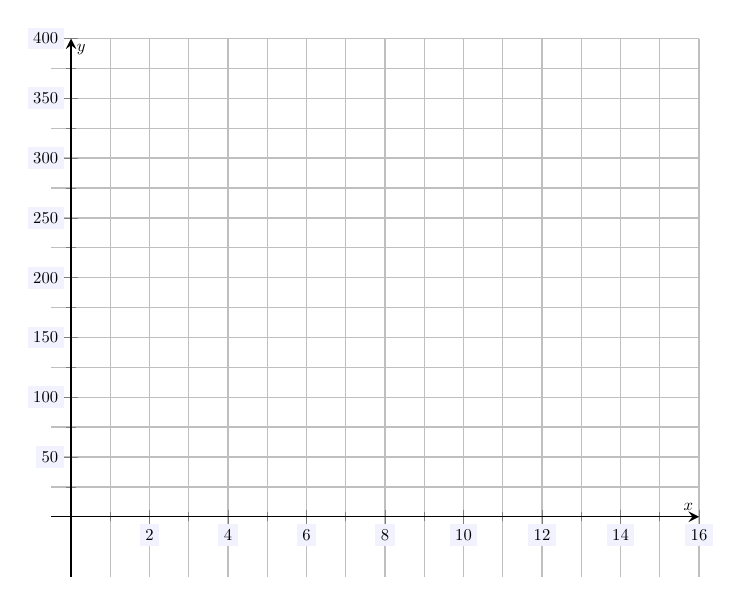
\begin{tikzpicture}[scale=1.2,every node/.style={scale=0.5}]
	\begin{axis}[
	grid=both,
	axis lines=middle,
	ticklabel style={fill=blue!5!white},
	xmin= -0.5, xmax=16,
	ymin= -50, ymax=400,
	xtick={0,2,...,16},
	ytick={0,50,...,400},
	minor x tick num = 1,
	minor y tick num = 1,
	xlabel=\(x\),ylabel=\(y\),
	]
%	\addplot[domain=-10.5:10.5,samples=2,line width=0.03cm] (x, 3/5*x - 3);
	\end{axis}
	\end{tikzpicture}
	}
	\] 


\end{document}